\subsection{Diagrama lógico/físico de datos}
\label{sec:erd}

Se presenta a continuación el diagrama que presenta el modelo lógico / físico como una variante simplificada del Diagrama Entidad-Relación \cite{chen1976entity}. Dicha variante ha sido obtenida de la notación ERwin/ERX2.0 \cite[p. 29]{song1995comparative} y \ac{SSADM} \cite[p. 193]{purchase2004comprehension}, así como del modo en el que lo generan sistemas de gestión de bases de datos como \program{Microsoft SQL Server} \cite[p. 30]{komputer2010shortcourse}, orientado a facilitar la lectura sin pérdida de semántica.

\begin{shaded}
No hay problema en utilizar el diagrama original de Chen o cualquier otro, siempre que esté justificado.
\end{shaded}

\begin{figure}[H]
\centering
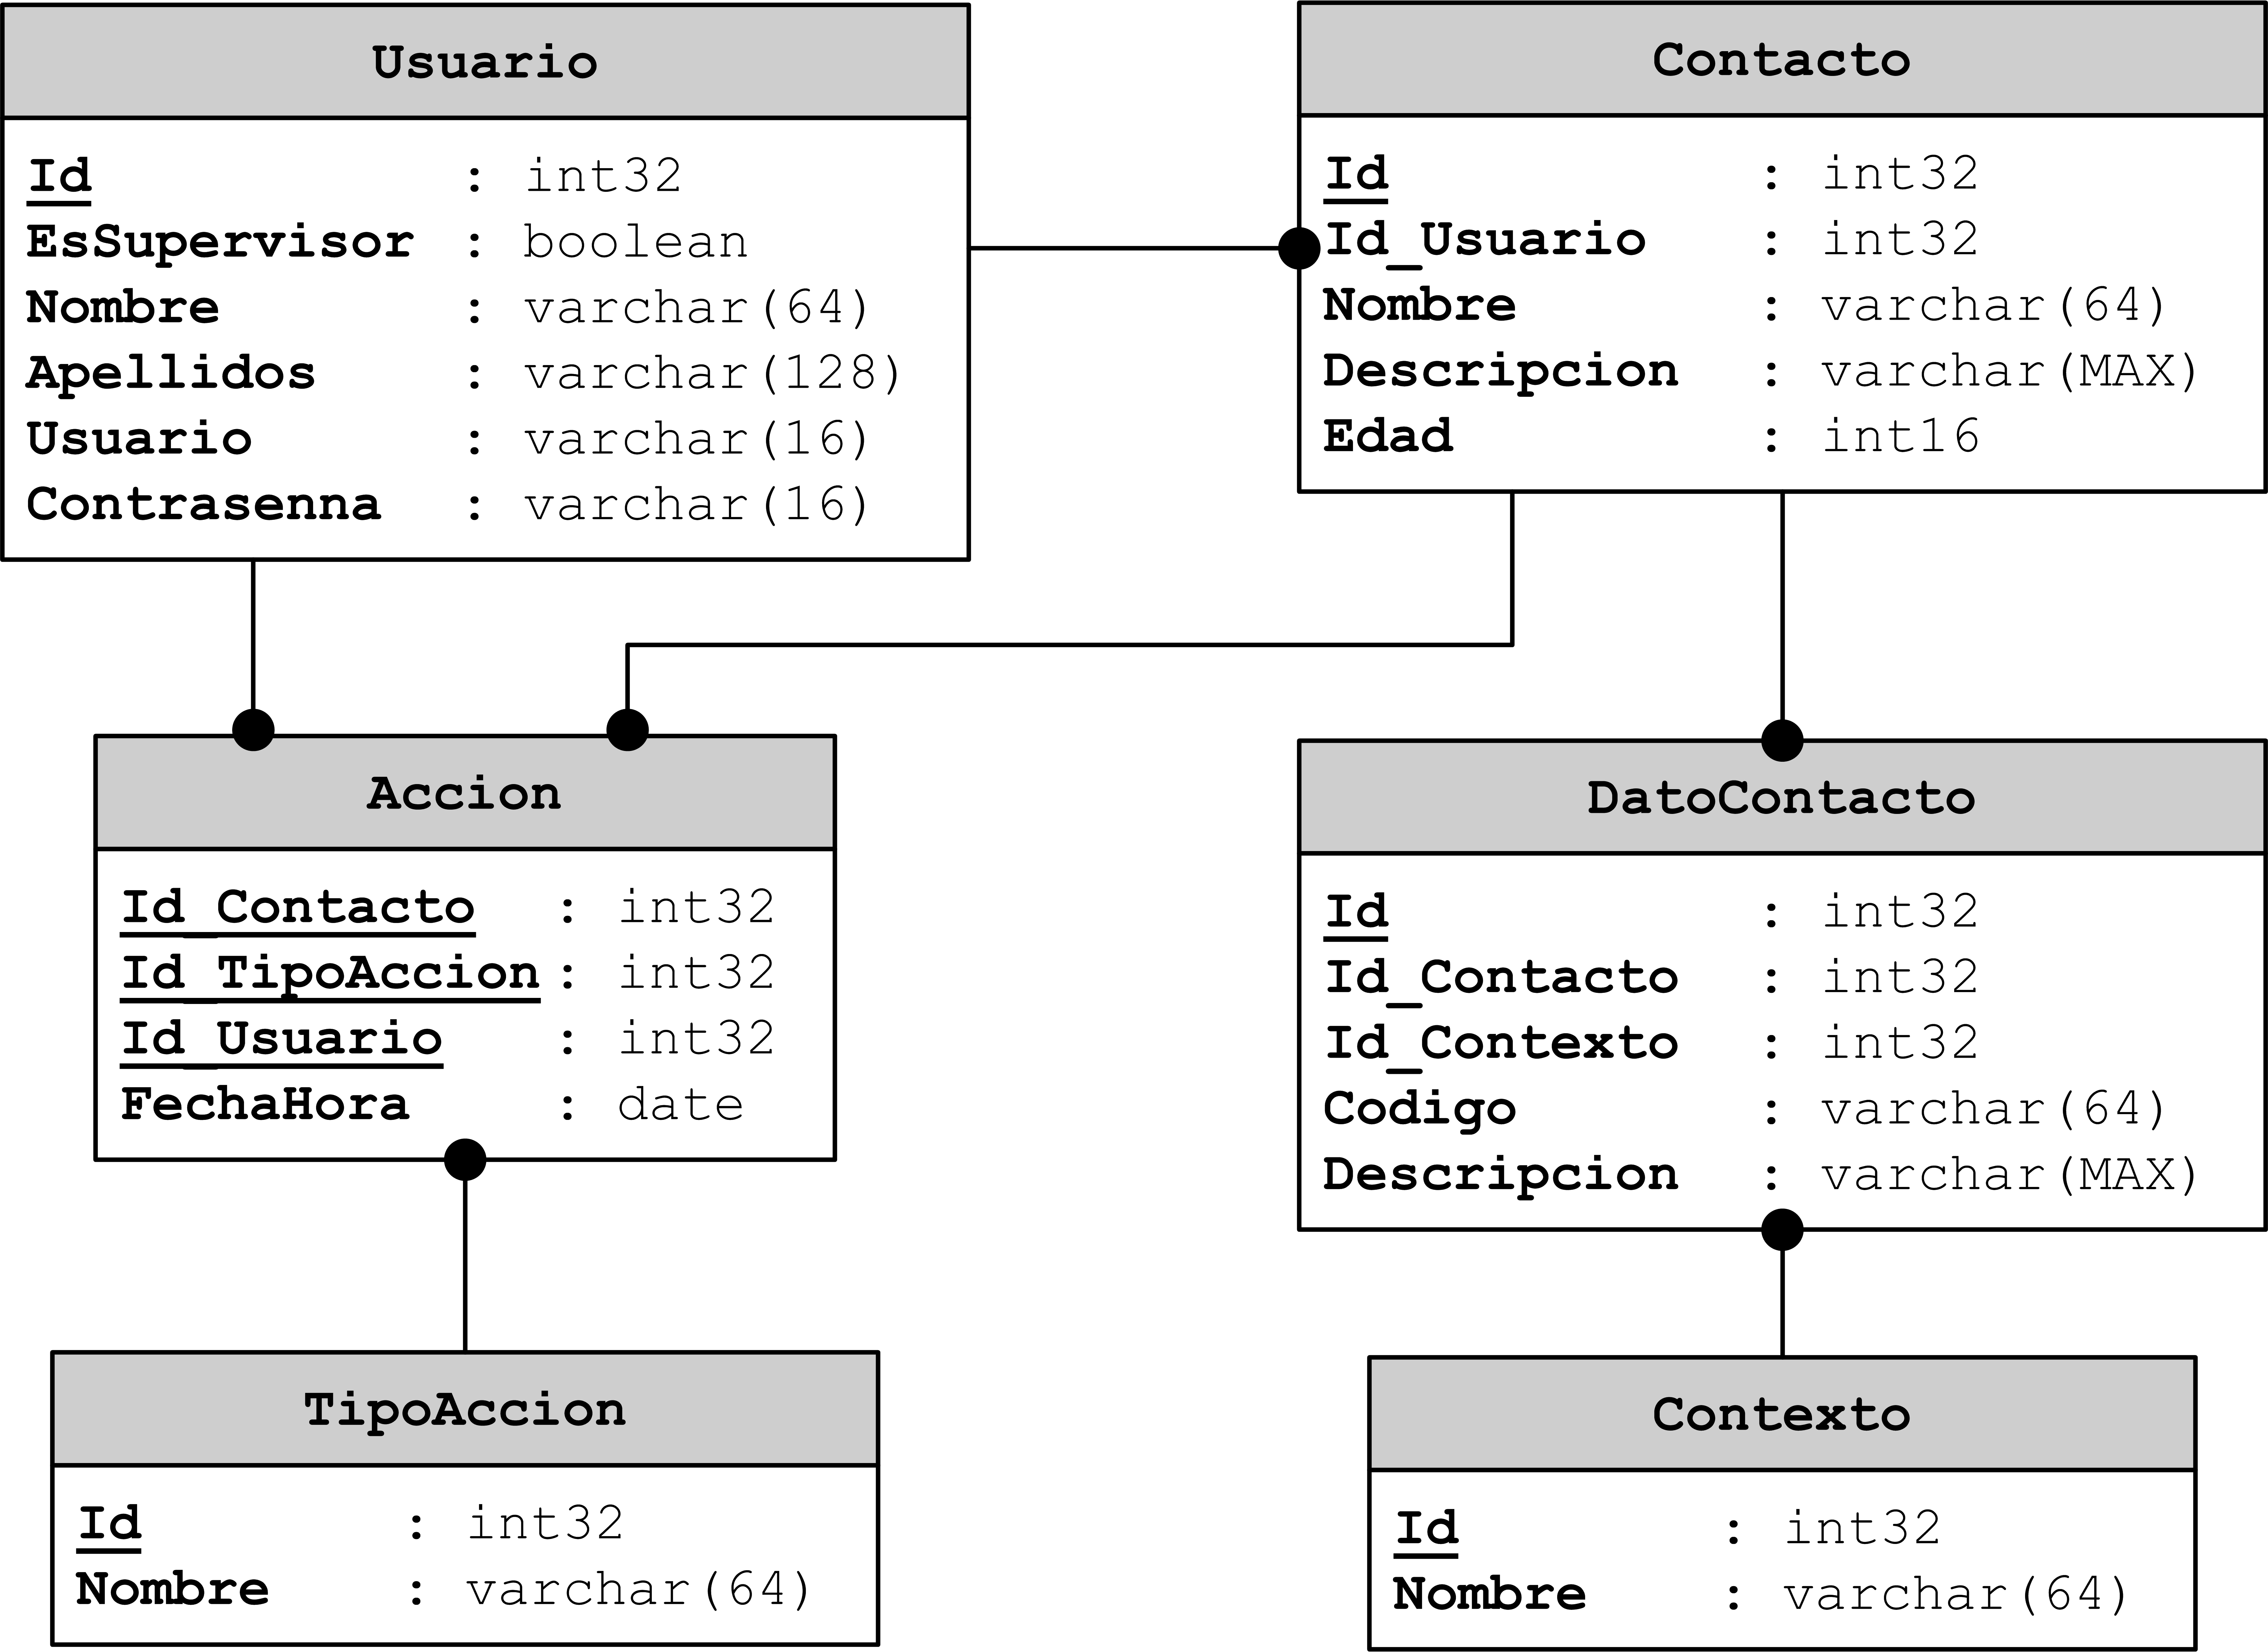
\includegraphics[scale=1]{erd.png}
\caption{Diagrama Entidad-Relación}
\label{fig:erd}
\end{figure}

\begin{shaded}
En caso de bases de datos relaciones, es interesante justificar la forma normal en la que se encuentra, sin entrar para ello en demasiado detalle sobre teoría de bases de datos.
\end{shaded}